\subsection*{Stage 1}
Assume that there exists a function $q : [0,1] \times [0,T] \to \mathbb{C},$ as smooth as we need, that satisfies the PDE and the IC. Applying Fourier transform to the PDE and using our preliminary work, we have
\begin{align*}
    \widehat{q_t} (x,t) &= - \widehat{q_{xxx}}(x,t) \\
    &=  \left(q_{xx}(0, t) + i \lambda q_x(0, t) - \lambda^2 q(0, t)\right) - e^{-i \lambda}  \left(q_{xx}(1, t) + i \lambda q_{x}(1, t) - \lambda^2 q(1, t)\right) + i \lambda^3 \widehat{q}(\lambda, t)
\end{align*}
which follows by preliminary work and rearrangement of terms. We subtract $ i \lambda^3 \widehat{q}(\lambda, t)$ from both sides of the above equation, and multiply the equaiton by $e^{- i \lambda^3 t}.$ Recalling the product rule for derivatives, we have on the left hand-side:
\[ 
e^{- i \lambda^3 t} \hat{q_t} (\lambda,t) - i \lambda^3 e^{- i \lambda^3 t} \hat{q}(\lambda, t) = \frac{d}{dt}  \left(e^{- i \lambda^3 t} \hat{q}(\lambda, t)\right),
\]
so that the above equation becomes
\begin{equation*}
\frac{d}{dt}  \left(e^{- i \lambda^3 t} \hat{q}(\lambda, t)\right) = e^{- i \lambda^3 t}\left(q_{xx}(0, t) + i \lambda q_x(0, t) - \lambda^2 q(0, t)\right) - e^{-i \lambda - i \lambda^3 t} \left(q_{xx}(1, t) + i \lambda q_{x}(1, t) - \lambda^2 q(1, t)\right).
\end{equation*}
Taking the integral from $0$ to $t$ yields
\begin{equation*}
\begin{aligned}
e^{- i \lambda^3 t} \widehat{q}(\lambda, t) - \widehat{q}(\lambda, 0) &= \int^t_0 e^{- i \lambda^3 s}\left(q_{xx}(0, s) + i \lambda q_x(0, s) - \lambda^2 q(0, s)\right) ~ \mathrm{d}s \\
&- \int^t_0 e^{-i \lambda - i \lambda^3 s} \left(q_{xx}(1, s) + i \lambda q_{x}(1, s) - \lambda^2 q(1, s)\right) ~ \mathrm{d}s.
\end{aligned}
\end{equation*}

Observe that $\widehat{q}(\lambda, 0)$ is the Fourier transform of the known function $q_0(x),$ so denote it as $\widehat{q_0}(\lambda).$ To simplify the notation, we further let 
\[ 
f_j(\lambda, X, t) := \int^t_0 e^{-i \lambda^3 s}~ \partial_x^j ~q(X,s)  ~\mathrm{d}s,
\]
so that we have 
\begin{equation}\label{GR}
\begin{aligned}
e^{- i \lambda^3 t} \hat{q}(\lambda, t) - \hat{q_0}(\lambda) &= \left(f_2(\lambda, 0, t) + i \lambda f_1(\lambda, 0, t) - \lambda^2 f_0(\lambda, 0, t)\right) \\
&- e^{-i \lambda} \left(f_2(\lambda, 1, t) + i \lambda f_1(\lambda, 1, t) - \lambda^2 f_0(\lambda, 1, t)\right). 
\end{aligned}\tag{GR}
\end{equation}
Since $\lambda$ and $t$ were arbitrary, the above equation, which we refer to as the \emph{Global Relation}, is valid for all $\lambda \in \mathbb{C}$ and all $t \in [0,T].$

Now solve for $\hat{q}(\lambda, t)$. Rearranging gives 
\begin{equation*}
\begin{aligned}
\hat{q}(\lambda, t) &= e^{i \lambda^3 t}\hat{q_0}(\lambda) + e^{i \lambda^3 t}\left(f_2(\lambda, 0, t) + i \lambda f_1(\lambda, 0, t) - \lambda^2 f_0(\lambda, 0, t)\right) \\
&- e^{i \lambda^3 t-i \lambda} \left(f_2(\lambda, 1, t) + i \lambda f_1(\lambda, 1, t) - \lambda^2 f_0(\lambda, 1, t)\right).
\end{aligned}
\end{equation*}
Applying inverse Fourier transform, we obtain
\begin{equation*}
\begin{aligned}
2\pi q(x, t) &= \int_{-\infty}^\infty e^{i\lambda x + i \lambda^3 t}\hat{q_0}(\lambda)\,d\lambda + \int_{-\infty}^\infty e^{i\lambda x + i \lambda^3 t}\left(f_2(\lambda, 0, t) + i \lambda f_1(\lambda, 0, t) - \lambda^2 f_0(\lambda, 0, t)\right)\,d\lambda \\
&- \int_{-\infty}^\infty e^{i\lambda x+i \lambda^3 t-i\lambda} \left(f_2(\lambda, 1, t) + i \lambda f_1(\lambda, 1, t) - \lambda^2 f_0(\lambda, 1, t)\right)\,d\lambda.
\end{aligned}
\end{equation*}
We need to deform the latter two contours of integration away from $\mathbb{R}$. We need the following definitions:
\begin{align*}
    \mathbb{C}^\pm &:= \{\lambda \in \mathbb{C}: \pm \mathrm{Im}(\lambda)>0\},\\
    D &:= \{\lambda \in \mathbb{C}: \mathrm{Re}(-i\lambda^3) < 0\}, \\
    E &:= \{\lambda \in \mathbb{C}: \mathrm{Re}(-i\lambda^3) > 0\},\\
    D^\pm & := D~\cap~\mathbb{C}^\pm,\\
    E^\pm & := E~\cap~\mathbb{C}^\pm.
\end{align*}
Orient the boundaries of these (unions of) sectors in the positive sense; the sector lies to the left of its boundary.
Note that if we let $\lambda = e^{i\theta}$ for $\theta \in \mathbb{R}$, then we can re-write sets $D$ and $E$ as
\begin{align*}
    &D = \{ e^{i\theta} \in \mathbb{C} \mid \cos(3\theta - \frac{\pi}{2}) < 0 \} \\
    &E = \{ e^{i\theta} \in \mathbb{C} \mid \cos(3\theta - \frac{\pi}{2}) > 0 \}. \\
\end{align*}
Refer to figure \ref{fig:intcontour} for a diagram of the sectors $D^{\pm}$ and $E^{\pm}$ on the complex plane.
\begin{figure}
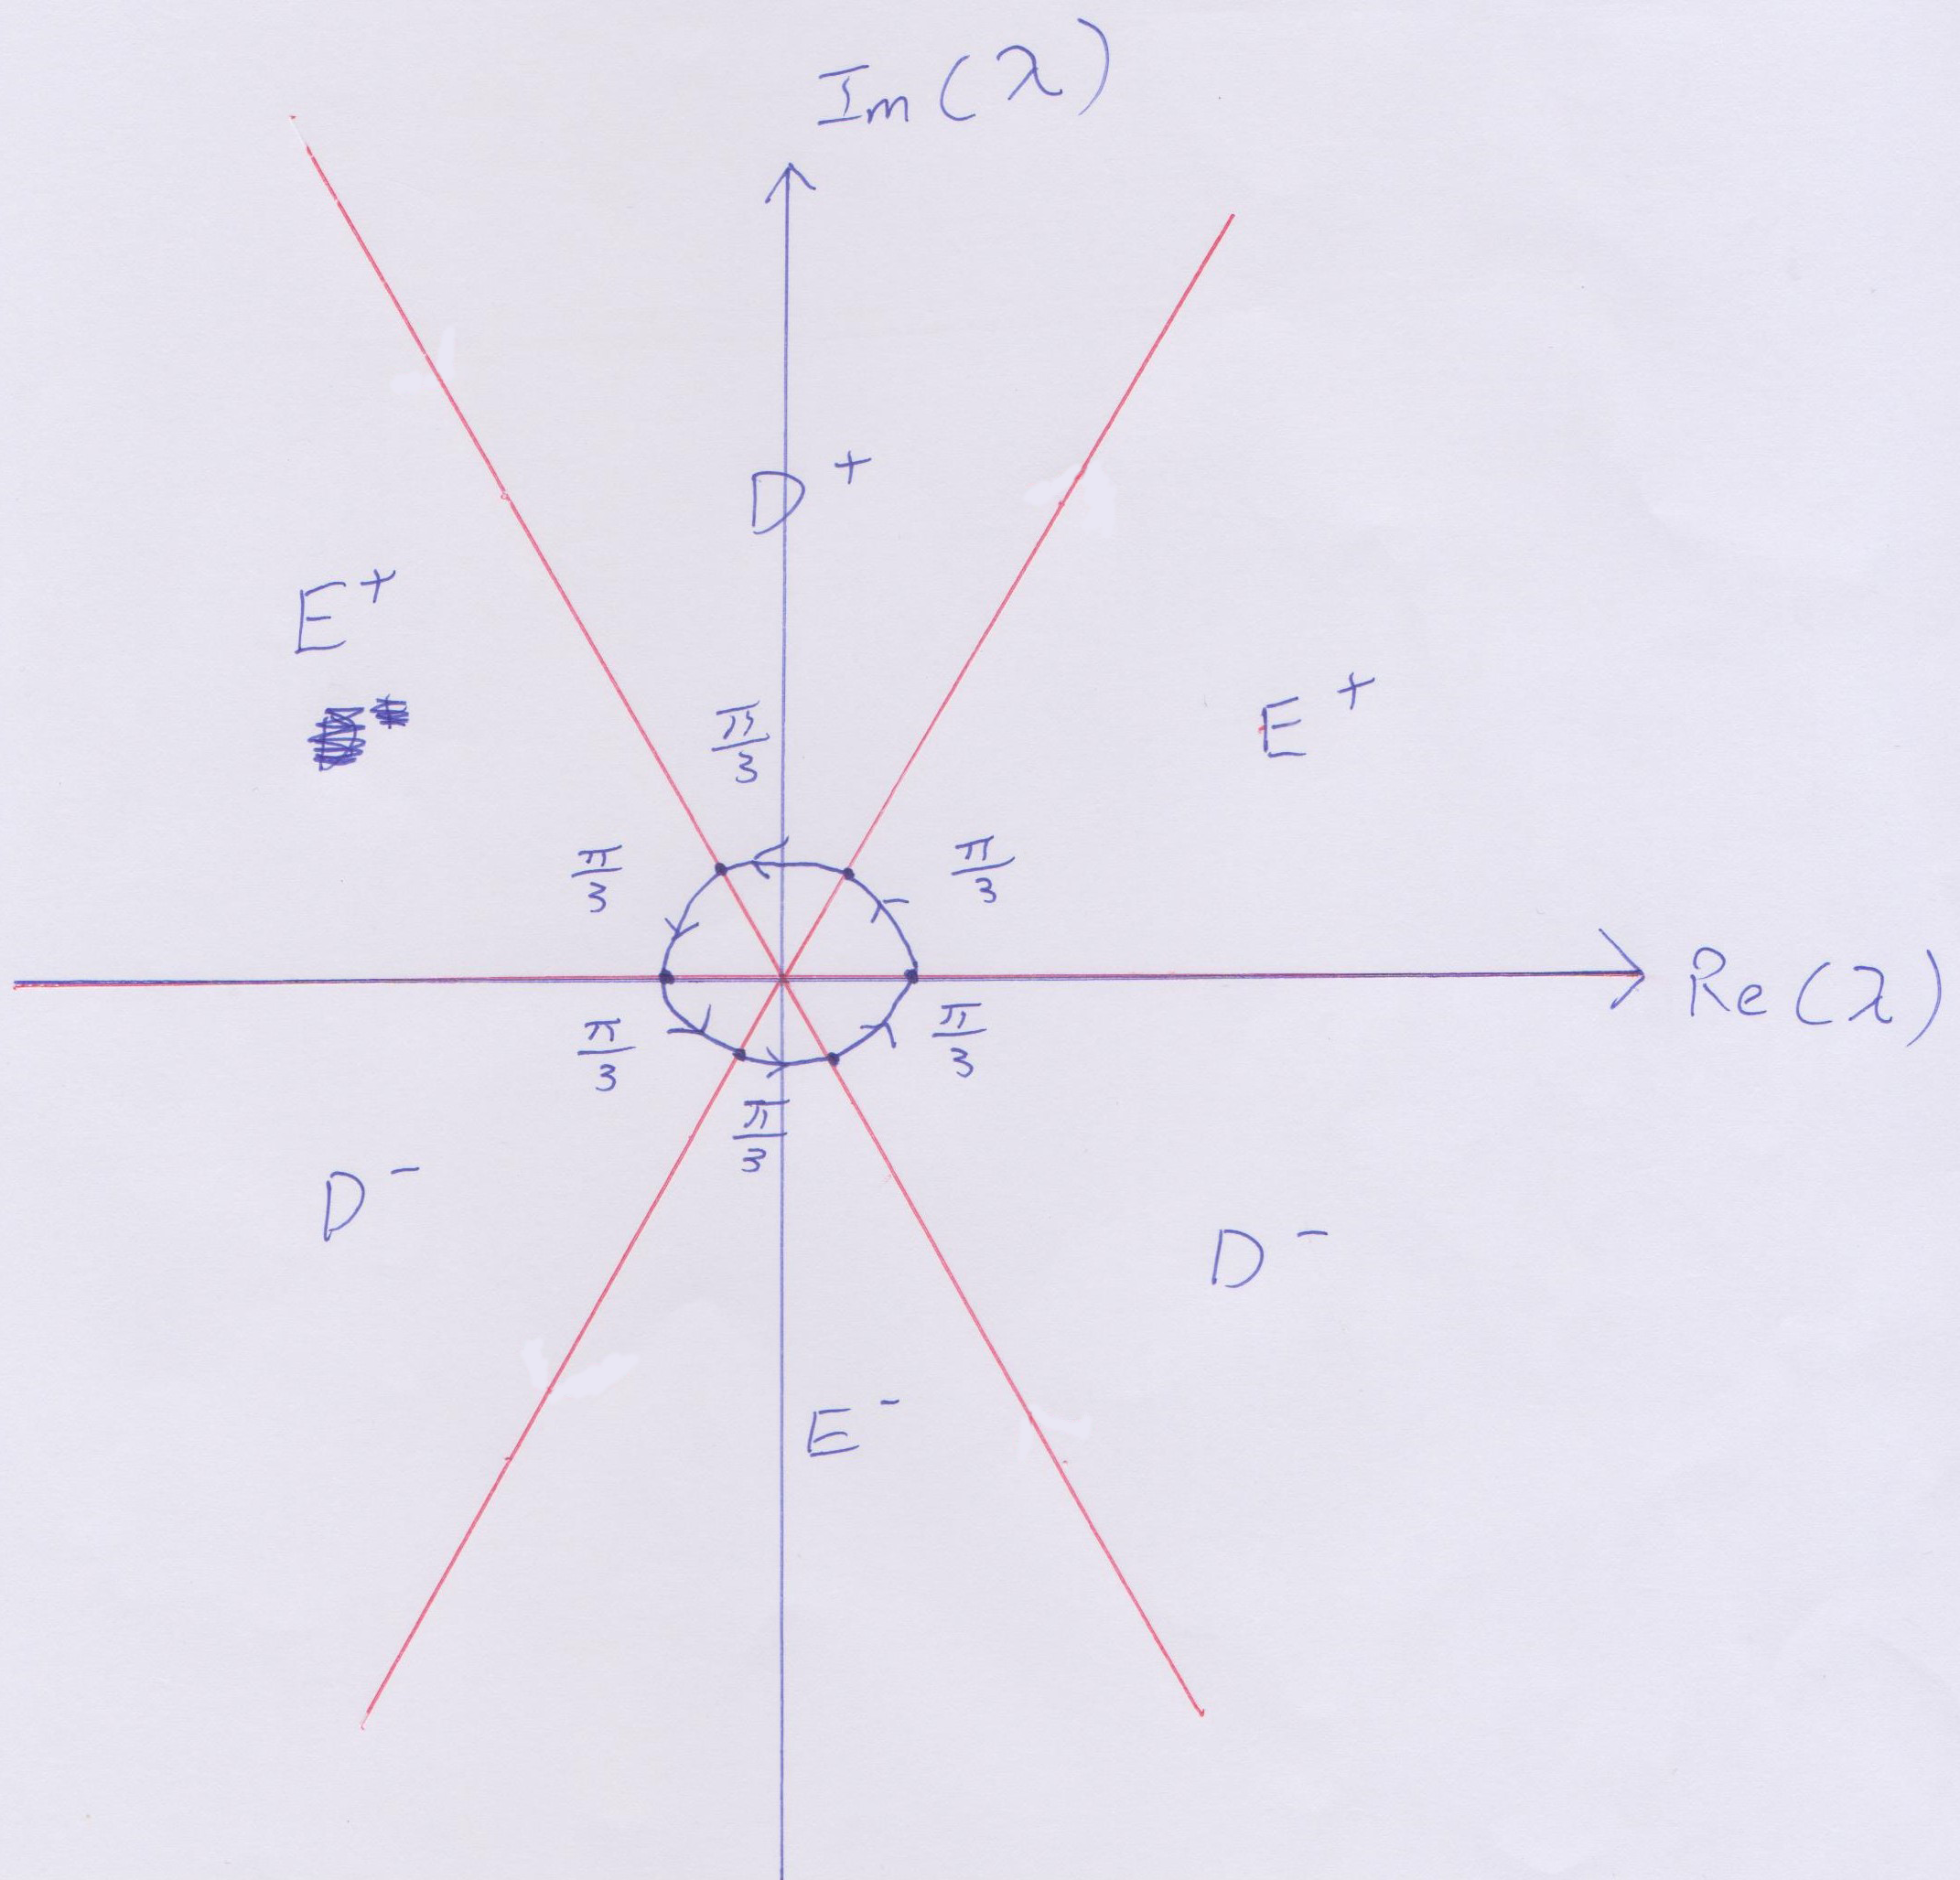
\includegraphics[width=\linewidth]{ImagesforFinalProblem/intcontour1.png}
\caption{A diagram showing the sectors $D^{\pm}$ and $E^{\pm}$ on the complex plane.}
\centering\label{fig:intcontour}
\end{figure}
Integration by parts gives
\begin{align*}
    e^{i\lambda^3t}f_j(\lambda,x,t) &= \int_0^t e^{i\lambda^3(t-s)}\partial_x^jg(x,s)\,ds\\
    &= -i\lambda^{-3}e^{i\lambda^3(t-s)}\partial_x^jg(x,s)\bigg|_{s=0}^{s=t} + i\lambda^{-3} \int_0^t e^{i\lambda^3(t-s)}\partial_s\partial_x^jg(x,s)\,ds\\
    &= \mathcal{O}(|i\lambda|^{-3}),
\end{align*}
uniformly in $\mathrm{arg}(\lambda)$ as $i\lambda \to \infty$ within $\mathrm{clos}(D)$. This implies that \[e^{i \lambda^3 t}\left(f_2(\lambda, x, t) + i \lambda f_1(\lambda, x, t) - \lambda^2 f_0(\lambda, x, t)\right) = \mathcal{O}(|i\lambda|^{-1}),\]
uniformly in $\mathrm{arg}(\lambda)$ as $i\lambda \to \infty$ within $\mathrm{clos}(D)$. Also, \[e^{i \lambda^3 t}\left(f_2(\lambda, x, t) + i \lambda f_1(\lambda, x, t) - \lambda^2 f_0(\lambda, x, t)\right)\]
is entire as $\partial_x^j(x,\cdot) \in L'[0,T]$. Hence, by Jordan's lemma,
\[\int_{E^+} e^{i \lambda^3 t+i\lambda x}\left(f_2(\lambda, x, t) + i \lambda f_1(\lambda, x, t) - \lambda^2 f_0(\lambda, x, t)\right)d\lambda = 0\]
for all $x > 0$.
Recalling the original integral, the above suggests that 
\begin{align*}
    \int_{-\infty}^{\infty} &e^{i \lambda^3 t+i\lambda x}\left(f_2(\lambda, 0, t) + i \lambda f_1(\lambda, 0, t) - \lambda^2 f_0(\lambda, 0, t)\right)d\lambda \\
    &= \left\{ \int_{-\infty}^{\infty} - \int_{E^+} \right\} e^{i \lambda^3 t+i\lambda x}\left(f_2(\lambda, 0, t) + i \lambda f_1(\lambda, 0, t) - \lambda^2 f_0(\lambda, 0, t)\right)d\lambda \\
    &= \int_{D^+} e^{i \lambda^3 t+i\lambda x}\left(f_2(\lambda, 0, t) + i \lambda f_1(\lambda, 0, t) - \lambda^2 f_0(\lambda, 0, t)\right)d\lambda.
\end{align*}
Similarly, by Jordan's lemma, 
\[\int_{E^-} e^{i \lambda^3 t+i\lambda x - i \lambda}\left(f_2(\lambda, x, t) + i \lambda f_1(\lambda, x, t) - \lambda^2 f_0(\lambda, x, t)\right)d\lambda = 0\]
for all $x > 0,$ so that 
\begin{align*}
    \int_{-\infty}^\infty &e^{i\lambda x+i \lambda^3 t-i\lambda} \left(f_2(\lambda, 1, t) + i \lambda f_1(\lambda, 1, t) - \lambda^2 f_0(\lambda, 1, t)\right)\,d\lambda \\
    &= - \int_{\infty}^{-\infty} e^{i\lambda x+i \lambda^3 t-i\lambda} \left(f_2(\lambda, 1, t) + i \lambda f_1(\lambda, 1, t) - \lambda^2 f_0(\lambda, 1, t)\right)\,d\lambda \\
    &= - \left\{ \int_{\infty}^{-\infty} - \int_{E^-} \right\} e^{i\lambda x+i \lambda^3 t-i\lambda} \left(f_2(\lambda, 1, t) + i \lambda f_1(\lambda, 1, t) - \lambda^2 f_0(\lambda, 1, t)\right)\,d\lambda \\
    &= -\int_{D^-} e^{i\lambda x+i \lambda^3 t-i\lambda} \left(f_2(\lambda, 1, t) + i \lambda f_1(\lambda, 1, t) - \lambda^2 f_0(\lambda, 1, t)\right)\,d\lambda.
\end{align*}
Through these deformations, we have arrived at the Ehrenpreis form:
\begin{equation*}\label{EFt}
\begin{aligned}
2\pi q(x, t) &= \int_{-\infty}^\infty e^{i\lambda x + i \lambda^3 t}\hat{q_0}(\lambda)\,d\lambda + \int_{D^+} e^{i \lambda^3 t+i\lambda x}\left(f_2(\lambda, 0, t) + i \lambda f_1(\lambda, 0, t) - \lambda^2 f_0(\lambda, 0, t)\right)d\lambda \\
&+\int_{D^-} e^{i\lambda x+i \lambda^3 t-i\lambda} \left(f_2(\lambda, 1, t) + i \lambda f_1(\lambda, 1, t) - \lambda^2 f_0(\lambda, 1, t)\right)\,d\lambda,
\end{aligned}\tag{EF$t$}
\end{equation*}
valid for $(x, t) \in (0,1) \times[0,T].$

By a similar argument, for all $\tau \in [t,T],$ we have  
\[ e^{i \lambda^3 t} \left(\int_{t}^{\tau} e^{- i \lambda^3 s}\left(q_{xx}(0, s) + i \lambda q_x(0, s) - \lambda^2 q(0, s)\right) ~ \mathrm{d}s \right) = \mathcal{O}(|i\lambda|^{-1})\]
uniformly in $\mathrm{arg}(\lambda)$ as $i\lambda \to \infty$ within $\mathrm{clos}(D),$ so
\[ \int_{D^+} e^{i \lambda^3 t+i\lambda x}\left(f_2(\lambda, 0, \tau) + i \lambda f_1(\lambda, 0, \tau) - \lambda^2 f_0(\lambda, 0, \tau)\right)d\lambda = 0\]
and 
\[ \int_{D^-} e^{i\lambda x+i \lambda^3 t-i\lambda} \left(f_2(\lambda, 1, \tau) + i \lambda f_1(\lambda, 1, \tau) - \lambda^2 f_0(\lambda, 1, \tau)\right)\,d\lambda = 0.\]
This yields
\begin{equation*} \label{EFtau}
\begin{aligned}
2\pi q(x, t) &= \int_{-\infty}^\infty e^{i\lambda x + i \lambda^3 t}\hat{q_0}(\lambda)\,d\lambda + \int_{D^+} e^{i \lambda^3 t+i\lambda x}\left(f_2(\lambda, 0, \tau) + i \lambda f_1(\lambda, 0, \tau) - \lambda^2 f_0(\lambda, 0, \tau)\right)d\lambda \\
&+\int_{D^-} e^{i\lambda x+i \lambda^3 t-i\lambda} \left(f_2(\lambda, 1, \tau) + i \lambda f_1(\lambda, 1, \tau) - \lambda^2 f_0(\lambda, 1, \tau)\right)\,d\lambda,
\end{aligned}\tag{EF$\tau$}
\end{equation*}
which holds for $(x,t) \in (0,1)\times[0,\tau],$ where $\tau \in [0,T].$
